\section{Theory}
Every laser consists of three main components, the gain medium, a pump source
and an optical cavity. 
Stimulated emission in the gain medium amplifies incoming light. For these atomic transitions,
which determine the laser spectrum, it is crucial to create population inversion in the 
gain medium. This is achieved by the pump source, which constantly supplies energy.
The amplification grows exponentially with the travel distrance of the photons through 
the gain medium. Therefore the gain medium is placed in a cavity consisting of two 
parallel reflecting elements so that the photons can pass the gain medium multiple times.

\subsection*{Atomic Transitions}
In atomic transitions between different discrete energy levels the three processes 
absorption, spontaneous emission and stimulated emission have to be distinguished, which are
shown schematically for a three-level system in Fig. \ref{fig:transitions}.
\begin{figure}
    \centering
    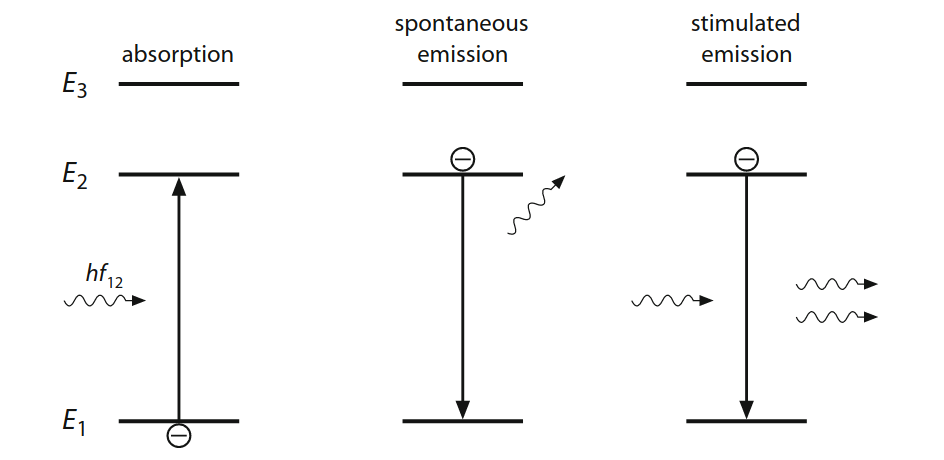
\includegraphics[width = 0.8\linewidth]{Bilder/transitions.png}
    \caption{Atomic transitions between two energy levels in a three-level system \cite{eichler}.}
    \label{fig:transitions}
\end{figure}
Spontaneous emission is the transition from a level of higher energy to a level of lower 
energy in which the energy difference between the two levels in released form of a photon.
If the transition is not spontaneous but induced by an incoming photon the process is 
called stimulated emission. 
Absorption occurs when an incoming photon causes a transition 
from the lower to the higher energy level and is absorbed in the process. 
In both stimulated emission and absorption the energy of the photon must correspond to the energy 
difference of the two energy levels.

Since the number of photons doubles in stimulated emission, light is amplified when 
stimulated emission occurs more often than spontaneous emission. For that, population inversion
is necessary and created by the pump source that adds energy to the 
system and thus increases the occupation probability of the upper level.                                                                                                                                                                                                                                                                                                                                                                                                                                                                                                                                                                                                         
Population inversion is not possible in a two-level system where only an equal occupation of 
both levels can be achieved because of the short relaxation time due to spontaneous emission.
Therefore at least three levels are needed. In this case, absorption occurs between the first (lowest)
and the third (highest) level, $E_1 \rightarrow E_3$. If the relaxation time of $E_3$ is 
much shorter than the relaxation time of $E_2$, a population inversion between the levels 
$E_1$ and $E_2$ is realised.

\subsection*{Diode Lasers}
In a diode laser, a semiconductor is used as the medium and an electric current is used as a 
pump source. 
%The conductivity of a material depends on the occupation of the conducting band and the 
In semiconducting materials the band gap between the conducting band and the valence band is very small. %with typical energies of a few electronvolts 
%with the Fermi level lying between those bands. 
At temperatures close to $T = 0 \text{ K}$, the conducting band is empty and the valence 
band fully occupied so that the material is isolating. 
By heating, electrons can be excited from the vanlence band to the conducting band, leaving
a hole in the valence band, and the material becomes conductive. 
The conductive properties of a semiconductor can also be increased by doping the material,
that is, introducing impurities into the crystal structure. These impurities, called dopants, are atoms with a 
different number of valence electrons than the semiconducting material and 
can either be donors and acceptors. 
Donors have an additional valence electron that can propagate freely in the conducting band,
the material is then n-doped. 
Acceptors are missing one valence electron and create holes as a positive charge carrier, the 
material is p-doped.
%If donors are introduced into the material, it is n-doted, if acceptors are introduced, it is p-doted.
In both cases the energy bands are shifted relative to the Fermi level, resulting in an 
increased conductivity.

Connecting p- and n-doped materials creates a p-n-junction as shown in fig. \ref{fig:semiconductor}. At the junction, free electrons from the n-doped layer diffuse 
to the p-doped layer where they recombine with holes. Conversely, holes from the p-doped layer diffuse into the n-doped layer
and recombine with electrons. This process creates a depletion layer (or space charge region) at the junction where the remaining
donor and acceptor atoms cause an electric field which opposes the diffusion process. 
Electric current can now only pass the p-n-juntion in one direction. Appliying a forward voltage to the 
p- and n-doped layers reduces the potential difference between the energy bands and creates a flow of electrons 
into the p-doped layer and a flow of holes into the n-doped layer. 
This results in a narrow region where population inversion is established and the laser can operate.

\begin{figure}
    \centering
    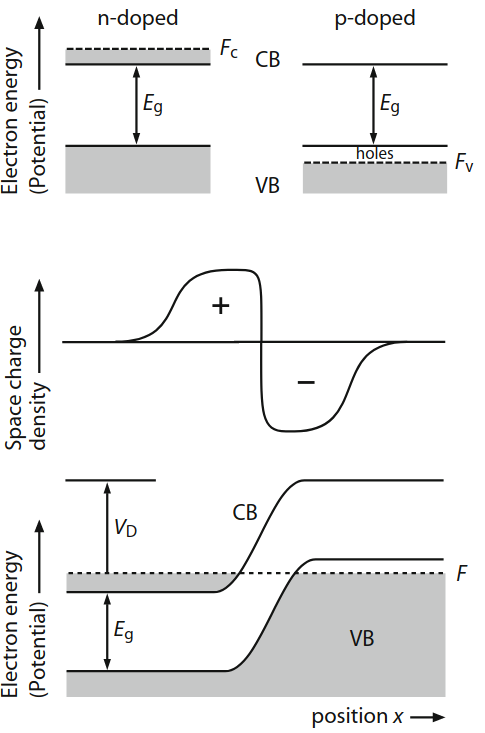
\includegraphics[width = 0.7\linewidth]{Bilder/semiconductor.png}
    \caption{Schematic illustration of a diode laser as a p-n-junction. 
    Top: Energy bands of seperated semiconductors with n- (left) and p-doping (right). $F_C$ and $F_V$ are the Fermi levels
    corresponding to the conduction (CB) and valence band (VB).
    Middle: Space charge densitiy distribution resulting from a diffusion of 
    electrons into the p-region and a diffusion of holes into the n-region 
    when connecting n- and p-type semiconductors.
    Bottom: Electron energy in the connected n- and p-doped areas \cite{eichler}.}
    \label{fig:semiconductor}
\end{figure}
%Light is emitted due to recombination of electron-hole pairs at the p-n-junction.
%The wavelength of the resonator corresponds to the band gap of the material.
%Two parallel layers of the medium, one of the only partially reflecting, function as the 
%resonator, or internal cavity.

\subsection*{Diode Chip and Cavities}
The schematic design of a diode chip is shown in fig. \ref{fig:design}.
\begin{figure}
    \centering
    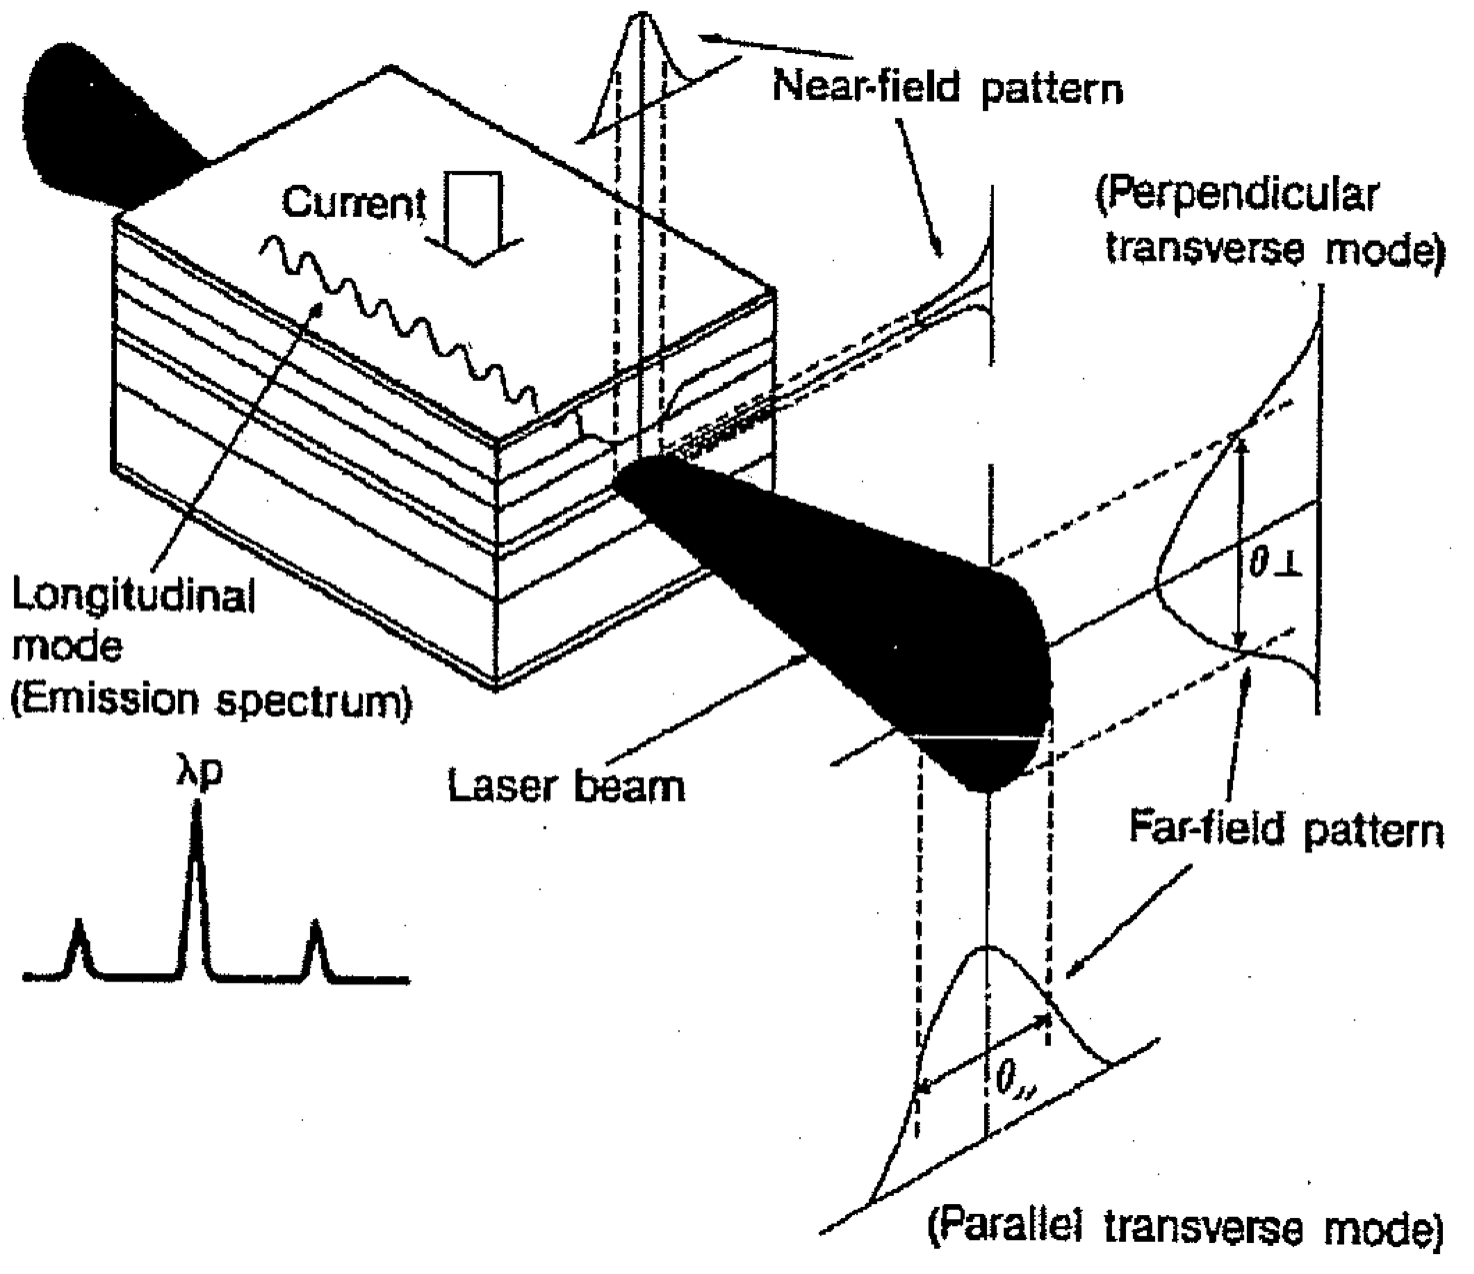
\includegraphics[width = 0.6\linewidth]{Bilder/design.jpeg}
    \caption{Schematic illustration of a laser diode chip \cite{sample}.}
    \label{fig:design}
\end{figure}
P- and n-doped layers are of different materials, this hetero structure serves as an optical wave guide.
The ends of the the diode chip are partially reflecting, forming the internal cavity. Inside the cavity a standing
wave emerges and the laser can emit in a single longitudinal cavity mode. 
The output beam is elliptical and strongly diverging. Therefore a lens is placed behind the laser that collimates
the beam.  To reduce the large linewidth and to increase the frequency stability an additional external cavity
is used. It is given by a diffraction grating that is placed behind the lens as shown in fig. \ref{fig:cavities}
\begin{figure}
    \centering
    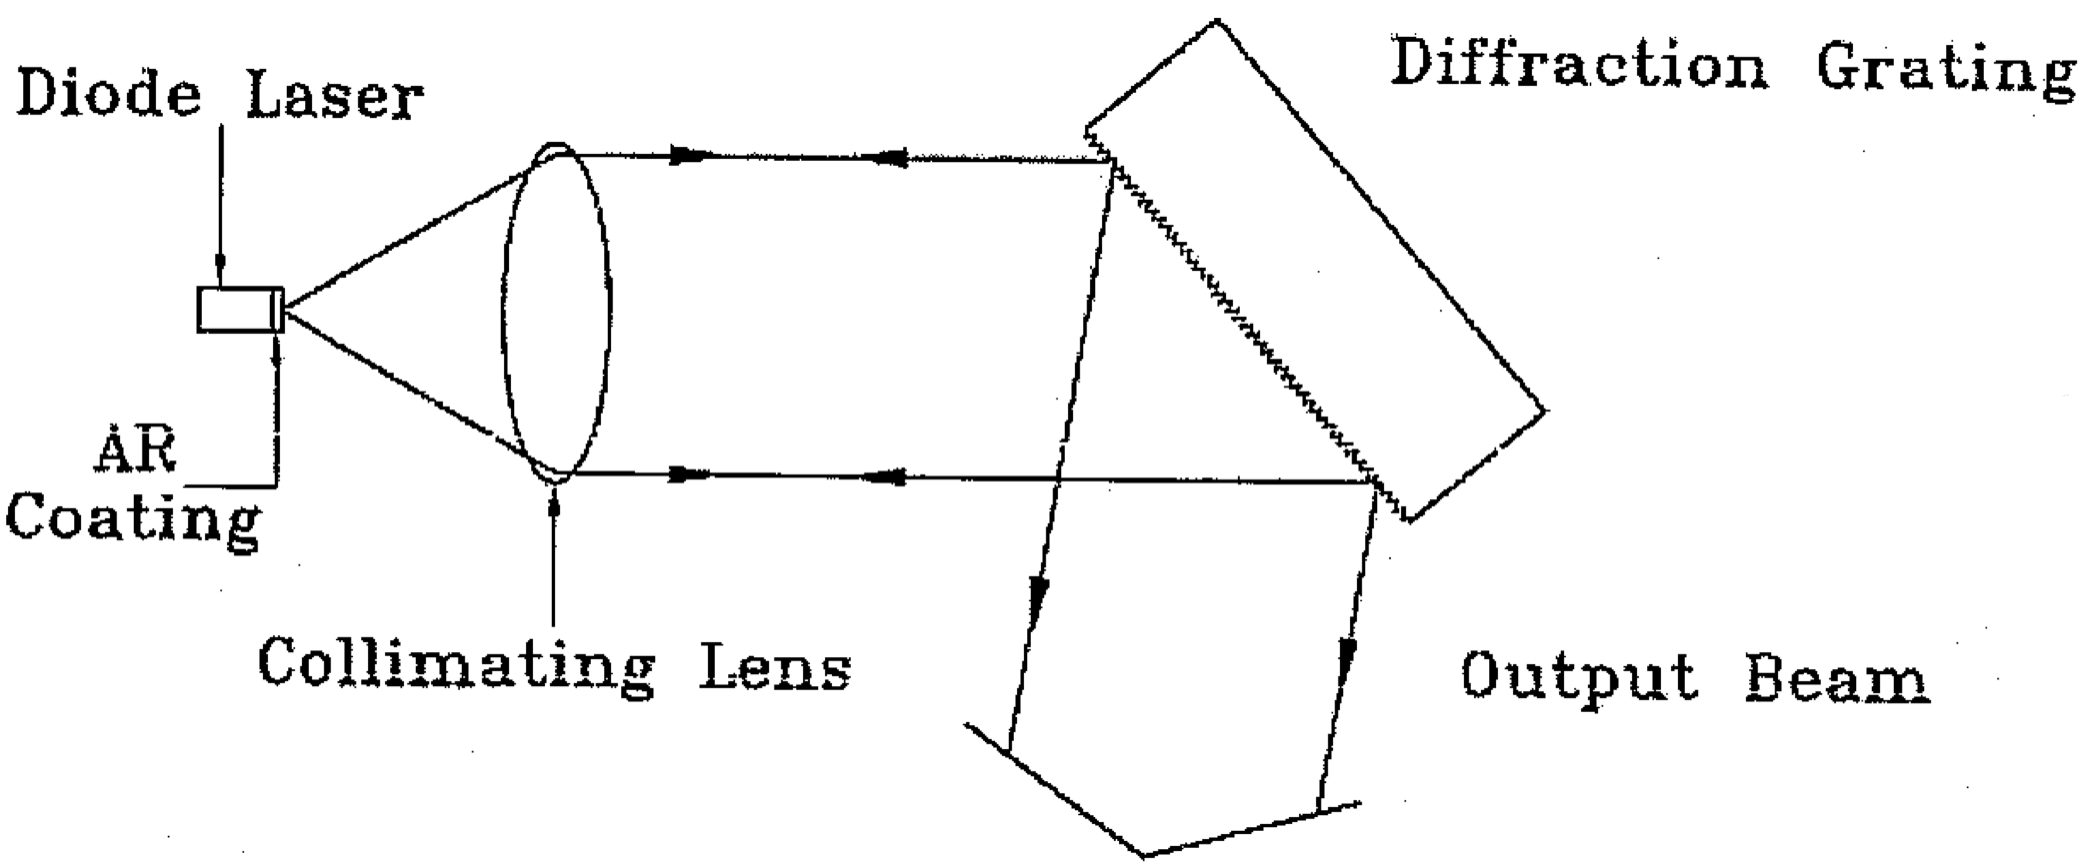
\includegraphics[width = 0.8\linewidth]{Bilder/cavities.png}
    \caption{Schematic illustration of the laser setup and the external cavity \cite{sample}.}
    \label{fig:cavities}
\end{figure}
With the grating, the first diffraction mode of the laser light is reflected back into the diode chip. By stimulated 
emission it increases the frequency stability. The frequency of the reflected light depends on the rotation angle of 
the grating, allowing for a frequency selection.

\subsection*{Laser Tuning}
The frequency of the laser light depends on various factors. The laser operates at the mode frequency with the 
highest net gain, that is, the difference of stimulated emission and optical losses.
The different contributions to the net gain are shown in fig. \ref{fig:netgain}.
\begin{figure}
    \centering
    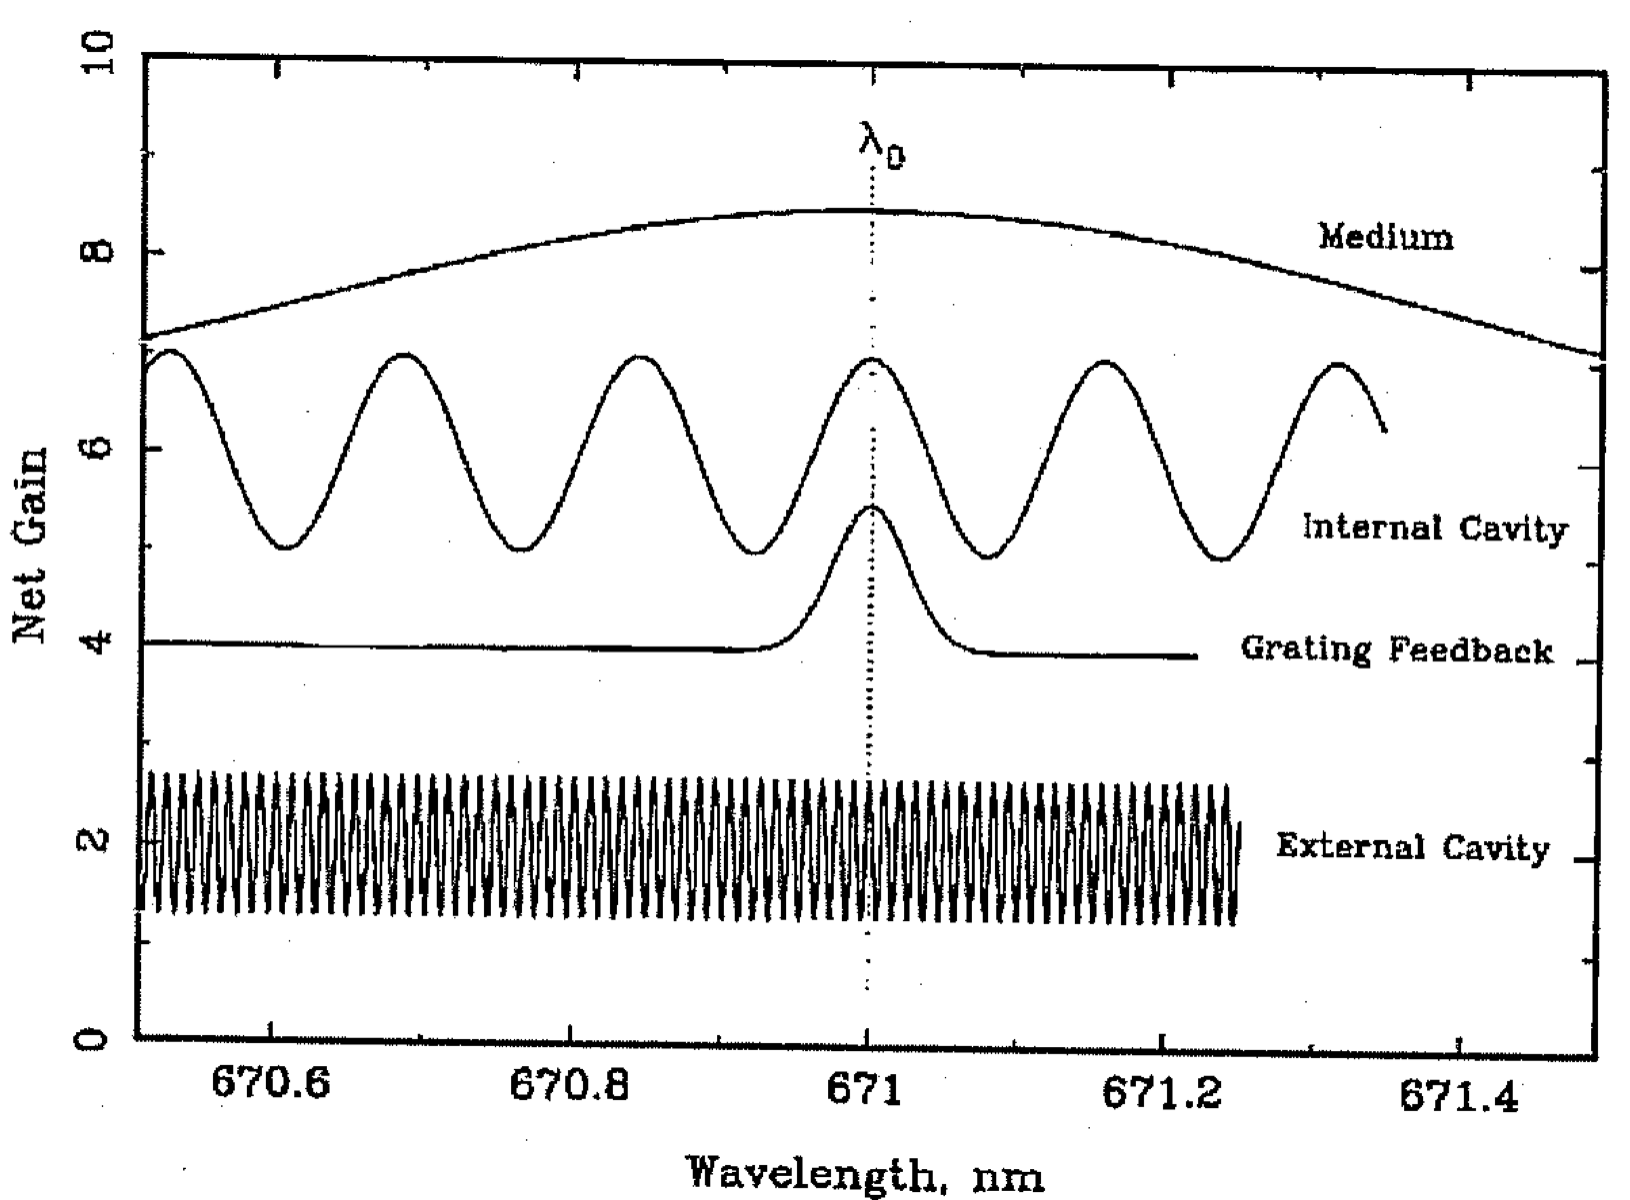
\includegraphics[width = 0.6\linewidth]{Bilder/netgain.png}
    \caption{Different contributions to the net gain of an arbitrary laser as a function of wavelength \cite{sample}.}
    \label{fig:netgain}
\end{figure}
%\subsubsection*{Medium Gain}
The medium gain depends on the band gap of the semiconductor material used and shows a broad peak. The 
peak position depends mainly on the laser temperature.
The internal cavity has a normal mode structure and thus an effective frequency-dependent net gain function that is 
periodic in frequency. The internal cavity gain funtion shifts in frequency with changes in the diode temperature.
The maximum gain of both medium and the internal cavity modes depends on the temperature of the diode that is affected by 
the applied current. Higher diode temperatures correspond to a shift to longer wavelengths. The shift rate however differs 
which leads to "mode hops" to different peaks of the cavity gain function.
The net gain also depends on the grating feedback, giving a single peak whose position depends on the grating angle, and
the external cavity, similar to the internal cavity.

\subsection*{Rubidium Absorption Spectrum}
Rubidum is an alkali metal with atomic number 37. There are two Rubidium isotopes that occur naturally on earth, 
${}^{87}\text{Rb}$ and ${}^{85}\text{Rb}$ of which only ${}^{85}\text{Rb}$ is stable.
If the laser emits light at a wavelength of $780 \, \text{nm}$, the spectrum of Rubidium can be observed. The spectrum
and the corresponding atomic transitions are shown in fig. \ref{fig:rubidium}.
\begin{figure}
    \centering
    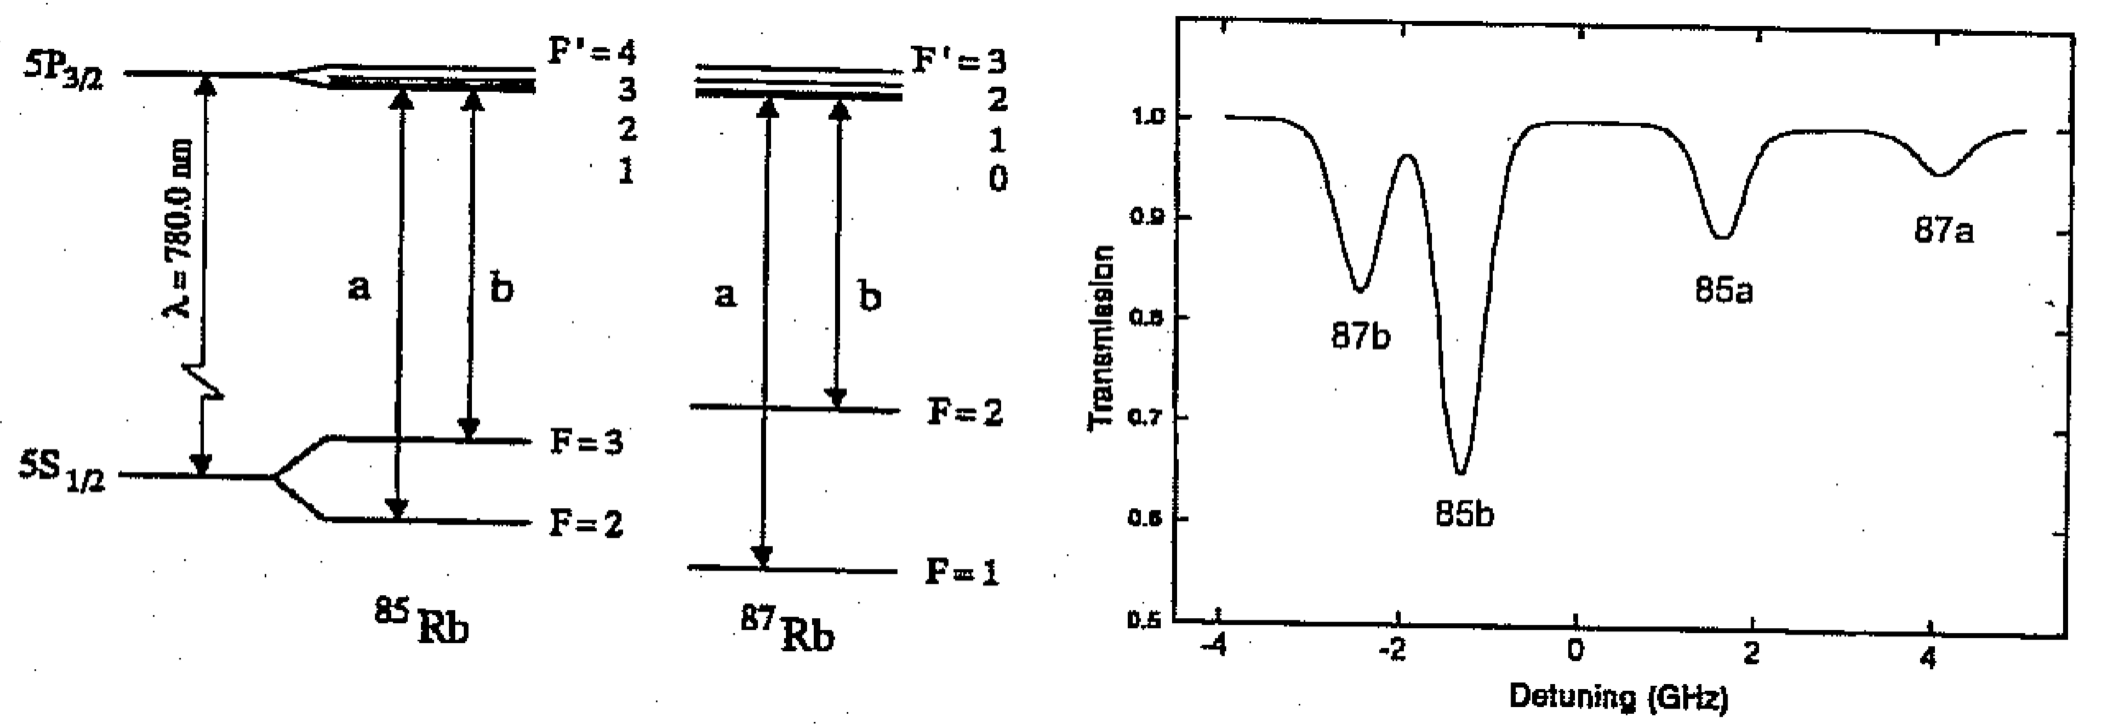
\includegraphics[width = \linewidth]{Bilder/rubidium.png}
    \caption{Schematic of the atomic transitions in Rubidium and the absorption spectrum \cite{sample}.}
    \label{fig:rubidium}
\end{figure}